\documentclass[11pt,a4paper]{article}
\usepackage[OT4]{polski}
\usepackage[utf8]{inputenc}
\usepackage[inner=2.5cm,outer=2.5cm, tmargin=2.5cm,bmargin=2.5cm]{geometry}
\usepackage{amsmath}
\usepackage{relsize,amsfonts}
\usepackage{enumitem}
\usepackage{graphicx}


  
\title{Bazy Danych\\\large \medskip Projekt\\}
\author{Mateusz Perciński Z59827}
\date{9 czerwca 2017}

\begin{document}

\maketitle

\section*{Treść projektu}
Zadanie zakłada zaprojektowanie i zaimplementowanie encji oraz relacji bazy danych aplikacji do nauki słówek, a także stworzenie podstawowych mechanizmów dynamicznych, które mogłyby znaleźć się w aplikacji tego typu. Dodatkowo, projekt zakłada napisanie prostej aplikacji w języku Java komunikującej się z bazą danych. 

\section{Projekt tabel}
Projekt bazy danych zakładał zbudowanie jak najabardziej elastycznej bazy danych. Założono możliwość dowolnego definiowania kursów na podstawie ich poziomu trudności, czy przynależności do kategorii(lub podkategorii - kategorie są połączone ze swoim nadkategoriami relacją unarną). Kursy są realizowane przez użytkowników, a dane słówko jest przydzielone do realizacji wraz z datą najbliższej powtórki.\\
Zaprojektowano również zależności dynamiczne w postaci triggerów, np. automacznie obliczających ilość słów w nowoutworzonym kursie\\


\begin{figure}[ht!]
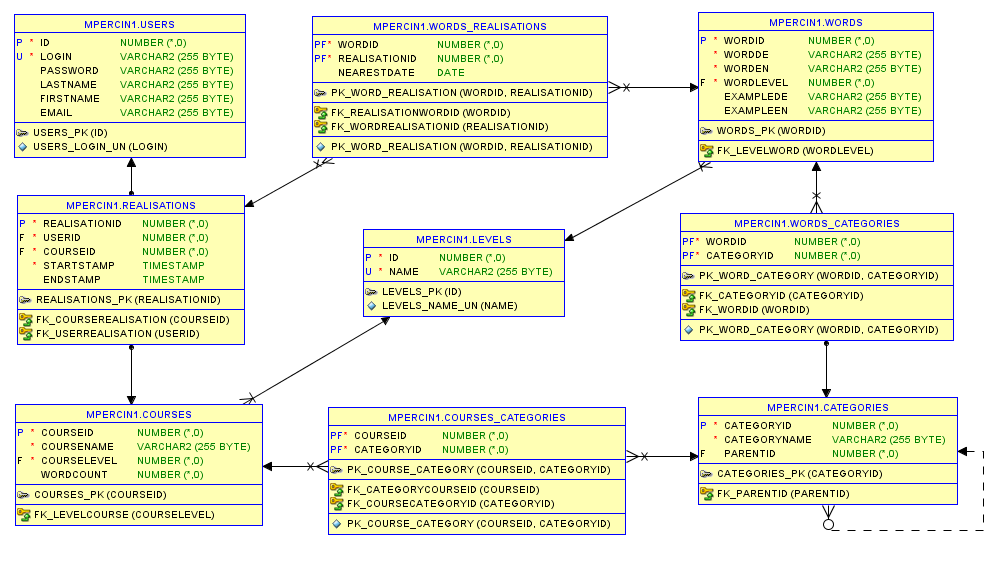
\includegraphics[width=\textwidth]{graphics/relational-model}
\caption{Model relacyjny bazy danych}
\label{fig:model}
\end{figure}

Załącznik \ref{attach:delete-db} to skrypt SQL kasujący istniejące tabele oraz sekwencje, natomiast załącznik \ref{attach:create-db} - budujący bazę danych od początku. Tworzy tabele, definiuje klucze własne oraz obce, czyli zależności relacyjne miedzy encjami. Rysunek \ref{fig:model} przedstawia model relacyjny projektowanej bazy danych.

\section{Wstawianie danych}
Dla każdej z tabel napisano polecenia INSERT INTO, wpisując małą ilość przykładowych unikalnych rekordów. Załącznik \ref{attach:insert} to skrypt SQL zawierający te polecenia.

\section{Generatory}
Załącznik \ref{attach:gen} to skrypt SQL zawierający definicję oraz wywołanie kilku generatorów danych o różnym stopniu skomplikowania.

\section{Triggery}
Załącznik \ref{attach:trigger} to skrypt SQL zawierający definicję oraz test triggerów. Realizują one nastepujące funkcjonalności:
\begin{itemize}
\item Sprawdzanie, czy klucz główny nie ma wartości NULL,
\item Sprawdzanie poprawności daty zakończenia kursu,
\item Automatyczne obliczanie ilości słów dla nowego kursu.
\end{itemize}

\section{Zapytania SQL}
Załącznik \ref{attach:select} zawiera zapytania do bazy danych, zaczynając od najprostszych, przez złączenia tablic, po bardziej skomplikowane z wykorzystanie zliczania oraz grupowania.

\section{Program w języku Java}
Program w języku Java wykonujący 4 podstawowe operacje DML: insert, update, delete, select, z wykorzystaniem JDBC API wykonano podczas laboratoriów. Załącznik \ref{attach:java} to fragment tego projektu, odpowiedzialny z konstrukcję i wywołanie poleceń SQL.

\section{Optymalizacja indeksów i Hinty}
Wykorzystanie indeksów zostało przedstawione w załączniku \ref{attach:index}, a zapytania z wykorzystaniem hintów w załączniku \ref{attach:hint}.


\section*{Spis załączników}
\addcontentsline{toc}{section}{Spis załączników} 
\begin{enumerate}[label=\arabic*,ref=\arabic*]
\item \label{attach:create-db} \textit{delete-db.sql} - skrypt SQL usuwający wszystkie tabele oraz sekwencje,
\item \label{attach:delete-db} \textit{create-db.sql} - skrypt SQL budujący hierarchię bazy danych
\item \label{attach:insert} \textit{insert.sql} - skrypt SQL wypełniający tablice przykładowymi danymi,
\item \label{attach:gen} \textit{generator.sql} - skrypt z definicjami generatorów danych PL/SQL,
\item \label{attach:trigger} \textit{trigger.sql} - skrypt z definicjami triggerów PL/SQL,
\item \label{attach:select} \textit{select.sql} - skrypt z zapytaniami SQL
\item \label{attach:java} \textit{DBTest.java} - fragment projektu w języku Java
\item \label{attach:index} \textit{index.sql} - skrypt SQL prezentujący użycie indeksów
\item \label{attach:hint} \textit{hint.sql} - skrypt SQL prezentujący użycie hintów
\end{enumerate}


\end{document}